\documentclass{beamer}
% use this instead for 16:9 aspect ratio:
%\documentclass[aspectratio=169]{beamer}
\usepackage{etex}
\reserveinserts{28}
\usetheme{ETHbeamer}

\colorlet{ETHcolor1}{ETHc}
\colorlet{ETHcolor2}{ETHc}

\author{Benjamin Ellenberger}
\institute{INI:  Institute of Neuroinformatics}

\title{Emergent gait periodicity in artificially evolved creatures on unknown terrains}

\date{2015-05-13}

% uncomment if you do not want to use a department logo
%\deplogofalse


\begin{document}

\titleframe

\section{Are we alone in the universe?}

\begin{frame}

  \frametitle{Contents}
  \tableofcontents[currentsection]
\end{frame}

% Life as it is vs. life as it could be
\begin{frame}

	\frametitle{Life as it is vs. life as it could be}

\end{frame}



\begin{frame}

	\frametitle{Applications}
	\begin{itemize}
	\item Build robots that are not only capable but also more adaptive (Engineering goal)
	\item Structures and strategies that always tend to evolve (Academic goal)
	\end{itemize}
\end{frame}

\section{Simple limiters theory}

% Simple limiter theory
\begin{frame}
	\frametitle{Simple limiters}
\end{frame}

%% Types of simple limiters in nature
\begin{frame}
	\frametitle{Simple limiters in nature}
	
	\begin{minipage}{.5\textwidth}
	\begin{itemize}
	\item Muscle length \& joint limits
	\item The weight of the limbs
	\item The relative position of limbs connected by joints (Direction of force applied to joints)
	\end{itemize}
\end{minipage}% This must go next to `\end{minipage}`
\begin{minipage}{.5\textwidth}
		%http://jonbarron.org/article/physiology-muscles
	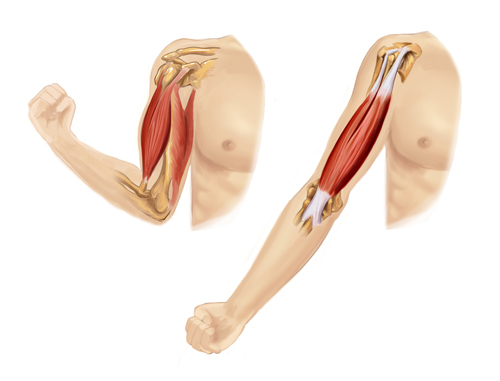
\includegraphics[width=1\textwidth]{figs/natural-limiter-arm-muscle.jpg}
\end{minipage}

\end{frame}

\begin{frame}
\frametitle{Simple limiters cont.}
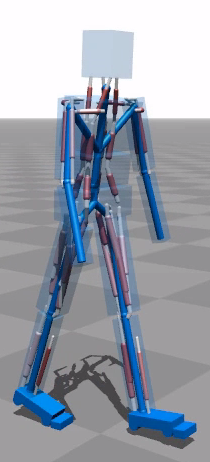
\includegraphics[width=0.2\textwidth]{figs/limiters/1.png}
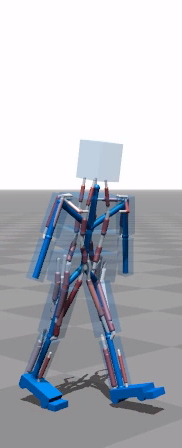
\includegraphics[width=0.2\textwidth]{figs/limiters/2.png}
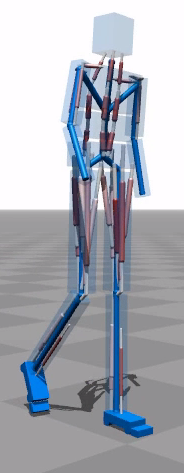
\includegraphics[width=0.2\textwidth]{figs/limiters/3.png}
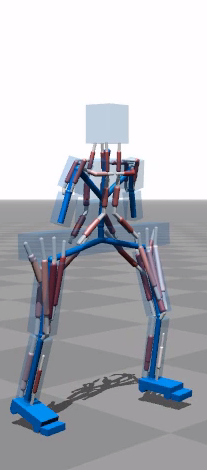
\includegraphics[width=0.2\textwidth]{figs/limiters/4.png}
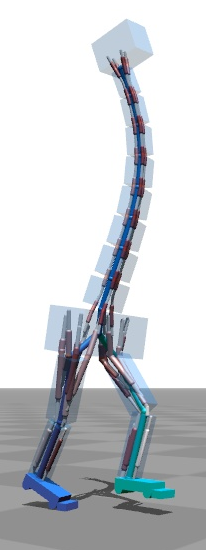
\includegraphics[width=0.2\textwidth]{figs/limiters/5.png}
\end{frame}

%% Will simple limiters be used if they do not need to be used
\begin{frame}
	\frametitle{In silico\footnote{In silico = in simulation}: Will they be used?}
	\begin{itemize}
	\item 
	\item 
	\end{itemize}
\end{frame}


\frame{

  \frametitle{Evolving Virtual Creatures}
  
  \begin{columns}
   \column{0.3\textwidth}
 \begin{itemize}
	     \item a
    	\item b
    	\item c
     \end{itemize}
     
     \column{0.6\textwidth}
      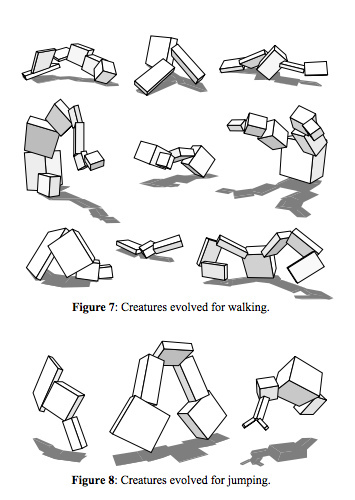
\includegraphics[width=2in, clip] {figs/creatures.jpg} 
  \end{columns}
  }
\note{}




\section{Methods}

\frame{

  \frametitle{Contents}
    \tableofcontents[currentsection]
}
\note{}

\subsection{Genetic language}
\frame{

  \frametitle{Genetic language}
  
Genotype:
\begin{tikzpicture}
   \foreach \c/\i/\t [count=\n] in  
        {blue!20/RootLimb/2,green!20/Limb1/1,orange!20/Limb2/0.8,red!20/Limb3/0.5} 
           \node[draw,fill=\c,minimum height=\t * 1.5cm,minimum width = \t * 1cm,xshift=\n* 2cm](N\n){\i} ;
\draw[dashed,->,line width=0.5mm] (N1.south) to [out=-50,in=-150] node[below] {Branch/2} (N2.south);
\draw[dashed,->,line width=0.5mm] (N2.north) to [out=50,in=150] node[above] {Branch/2} (N3.north);
\draw[dashed,->,line width=0.5mm] (N2.south) to [out=-50,in=-150] node[below] {Branch/2} (N4.south);

\end{tikzpicture}

  \begin{itemize}
\item \textbf{Limb} Part of creature body
\end{itemize}

  
  }
\note{}

\frame{
 \frametitle{Genetic language}
Phenotype:

% Set the overall layout of the tree
\tikzstyle{level 1}=[level distance=1cm, sibling distance=6cm]
\tikzstyle{level 2}=[level distance=1.5cm, sibling distance=1.4cm]

% Define styles
\tikzstyle{rl}=[draw,fill=blue!20,minimum height=3cm,minimum width=2cm]
\tikzstyle{l1}=[draw,fill=green!20,minimum height=1.5cm,minimum width=1cm]
\tikzstyle{l2}=[draw,fill=orange!20,minimum height=1.2cm,minimum width=0.8cm]
\tikzstyle{l3}=[draw,fill=red!20,minimum height=0.75cm,minimum width=0.5cm]

\begin{tikzpicture}[grow=down, sloped]
\node[rl] {RootLimb}
    child {
            node[l1] {Limb1}
            child {
                node[l2] {Limb2}
            }
            child {
                node[l3] {Limb3}
            }    
            child {
                node[l3] {Limb3}
            }
            child {
                node[l2] {Limb2}
            }
    }
    child {
            node[l1] {Limb1}
            child {
                node[l2] {Limb2}
            }
            child {
                node[l3] {Limb3}
            }    
            child {
                node[l3] {Limb3}
            }
            child {
                node[l2] {Limb2}
            }
    };
\end{tikzpicture}
  }
\note{}



\frame{

  \frametitle{Execution of creatures}
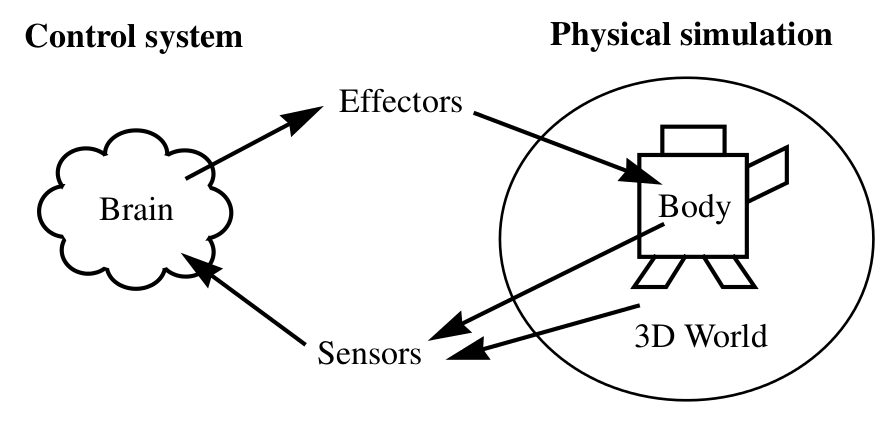
\includegraphics[width=2.3in, clip] {figs/brain-body-cycle.png}
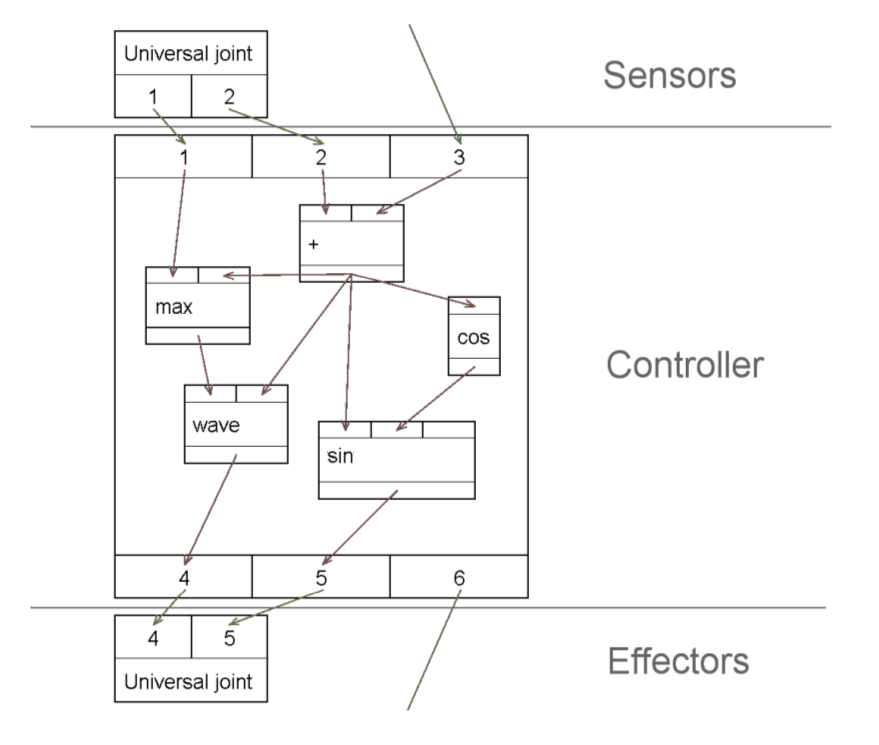
\includegraphics[width=2.5in, clip] {figs/execution.png}
  
  }
\note{}

\subsection{Fitness evaluation}
\frame{

  \frametitle{Fitness evaluation}

\begin{itemize}
\item Fitness evaluation framework
\item A creature is simulated for a certain evaluation time during which the fitness function measures the fitness of the creature
\item Evaluates multiple fitness functions at the same time and combines them linearly
\end{itemize}

  
  }
\note{}

\subsection{Evolution}
\frame{

  \frametitle{Evolution}

\begin{itemize}
\item Selection
\begin{itemize}
\item Only a certain percentage of creatures are selected for new generation
\end{itemize}
\item Cross-over
\begin{itemize}
\item Only certain percentage of creatures are allowed to breed
\end{itemize}
\item Mutation
\begin{itemize}
\item Other creatures are subject to mutation
\item Mutation of gene
\item Mutation of gene attributes
\item Mutation of gene branches
\end{itemize}
\item Successful creatures stay in the population and the population is refilled with new bred and mutated ones
\end{itemize}
  
  }
\note{}



\section{Simulations}

\frame{

  \frametitle{Contents}
    \tableofcontents[currentsection]
}
\note{}

\subsection{Velocity as the fitness function}
\frame{

  \frametitle{Velocity as the fitness function}

\begin{itemize}
\item Sampling of position over time
\item Moved distance in a certain time interval
\item Continuous average
\item Expectations: Some really moving creatures and some finding the exploit that only the main body has to move. \\(main body = first limb in phenotype)
\end{itemize}
  
  }
\note{}

\section{Meet \& Greet with the Creatures}

\frame{

  \frametitle{Creatures}
  \begin{figure}[tp]
    \centering
    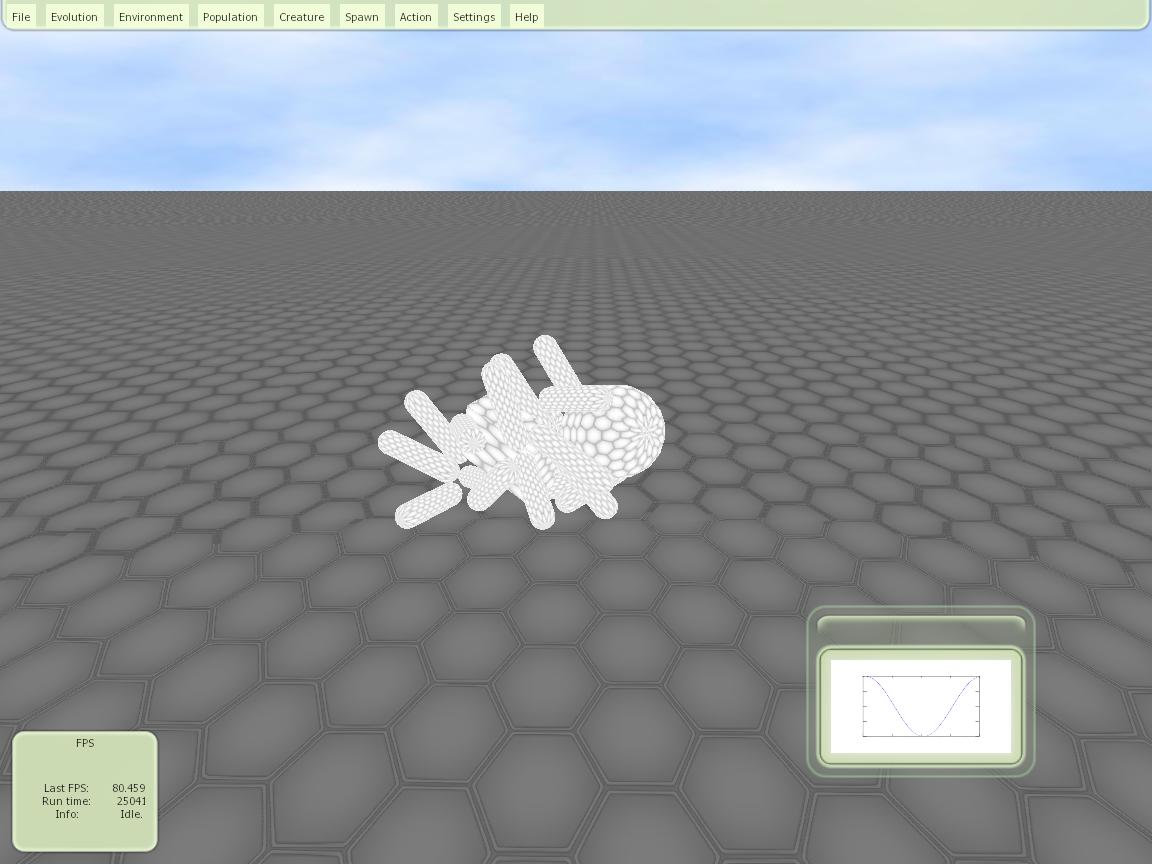
\includegraphics[width=3in, clip] {figs/creatures/Minemonics-05112015_184631057.jpg}
\end{figure}
  }
\note{}

\frame{

  \frametitle{Creatures}
  \begin{figure}[tp]
    \centering
    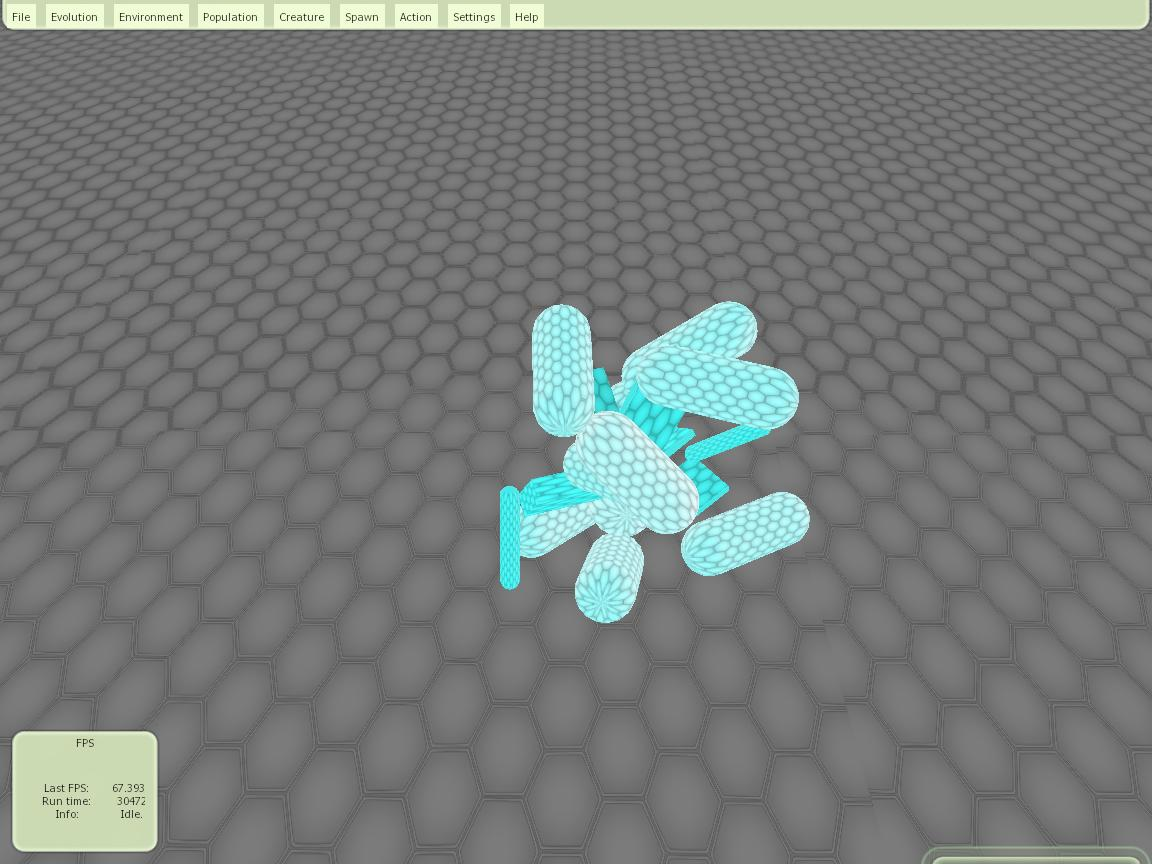
\includegraphics[width=3in, clip] {figs/creatures/Minemonics-05112015_190654362.jpg}
\end{figure}
  }
\note{}

\frame{

  \frametitle{Creatures}
  \begin{figure}[tp]
    \centering
    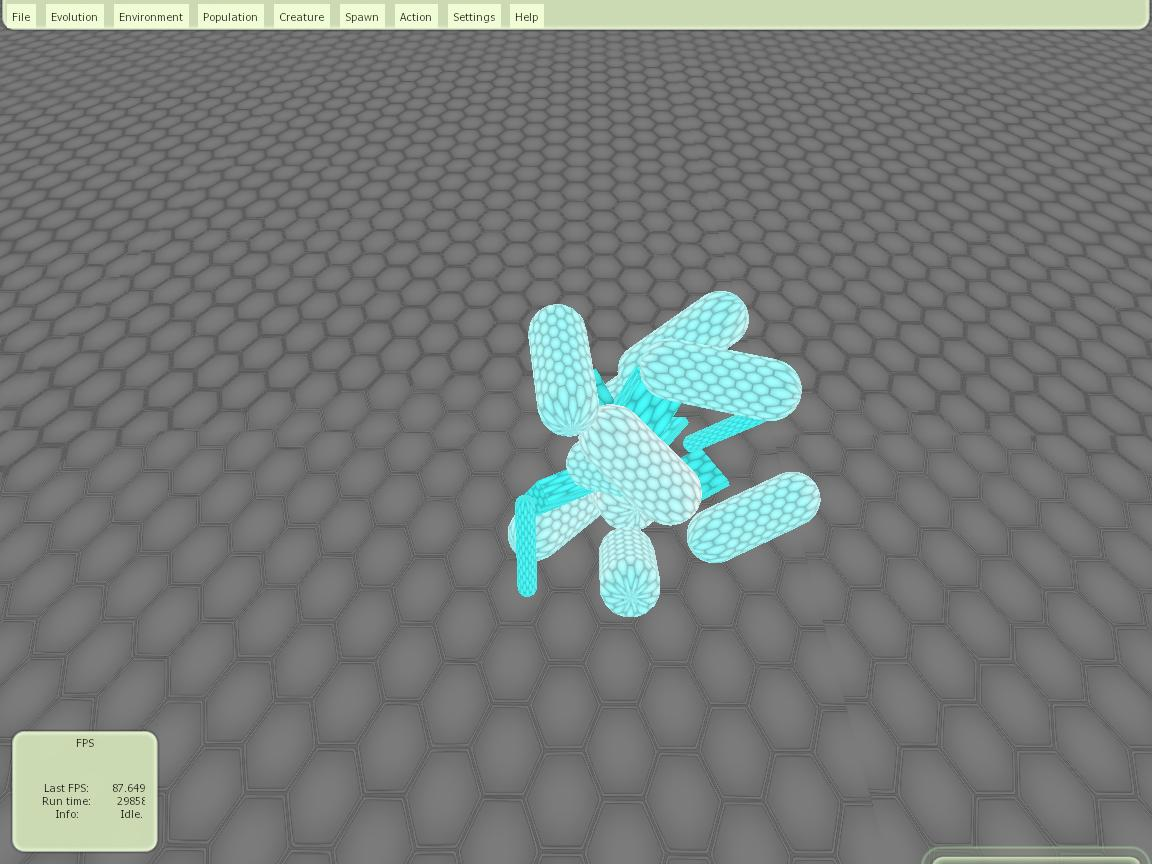
\includegraphics[width=3in, clip] {figs/creatures/Minemonics-05112015_190654779.jpg}
\end{figure}
  }
\note{}

\frame{

  \frametitle{Creatures}
  \begin{figure}[tp]
    \centering
    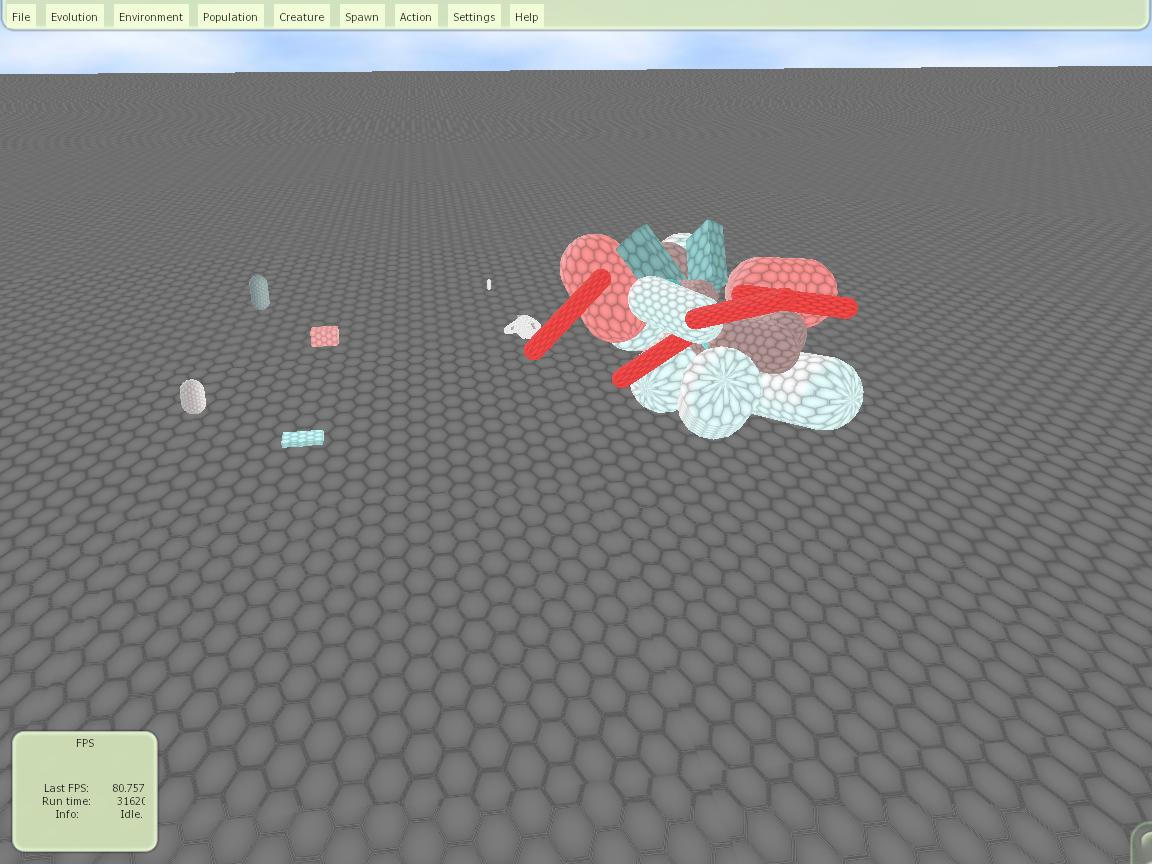
\includegraphics[width=3in, clip] {figs/creatures/Minemonics-05112015_190853660.jpg}
\end{figure}
  }
\note{}

\frame{

  \frametitle{Creatures}
  \begin{figure}[tp]
    \centering
    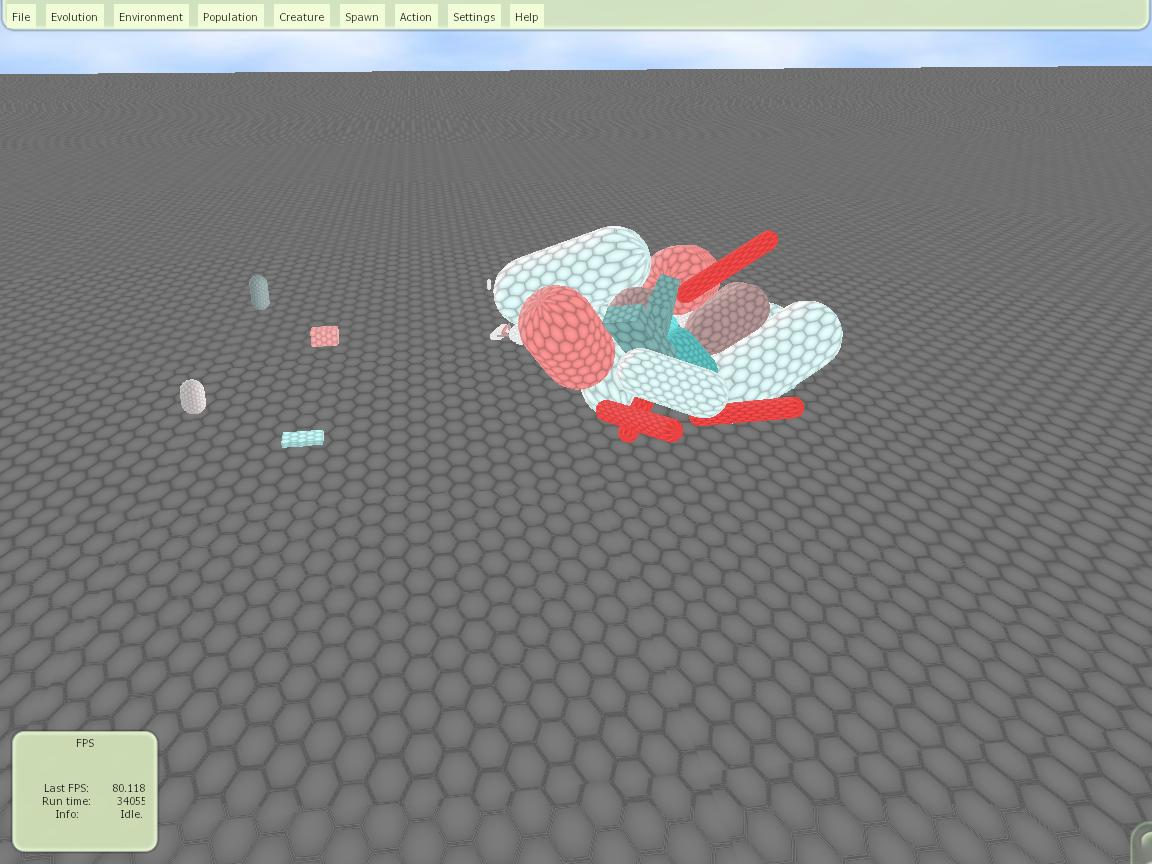
\includegraphics[width=3in, clip] {figs/creatures/Minemonics-05112015_190855124.jpg}
\end{figure}
  }
\note{}

\frame{

  \frametitle{Creatures}
  \begin{figure}[tp]
    \centering
    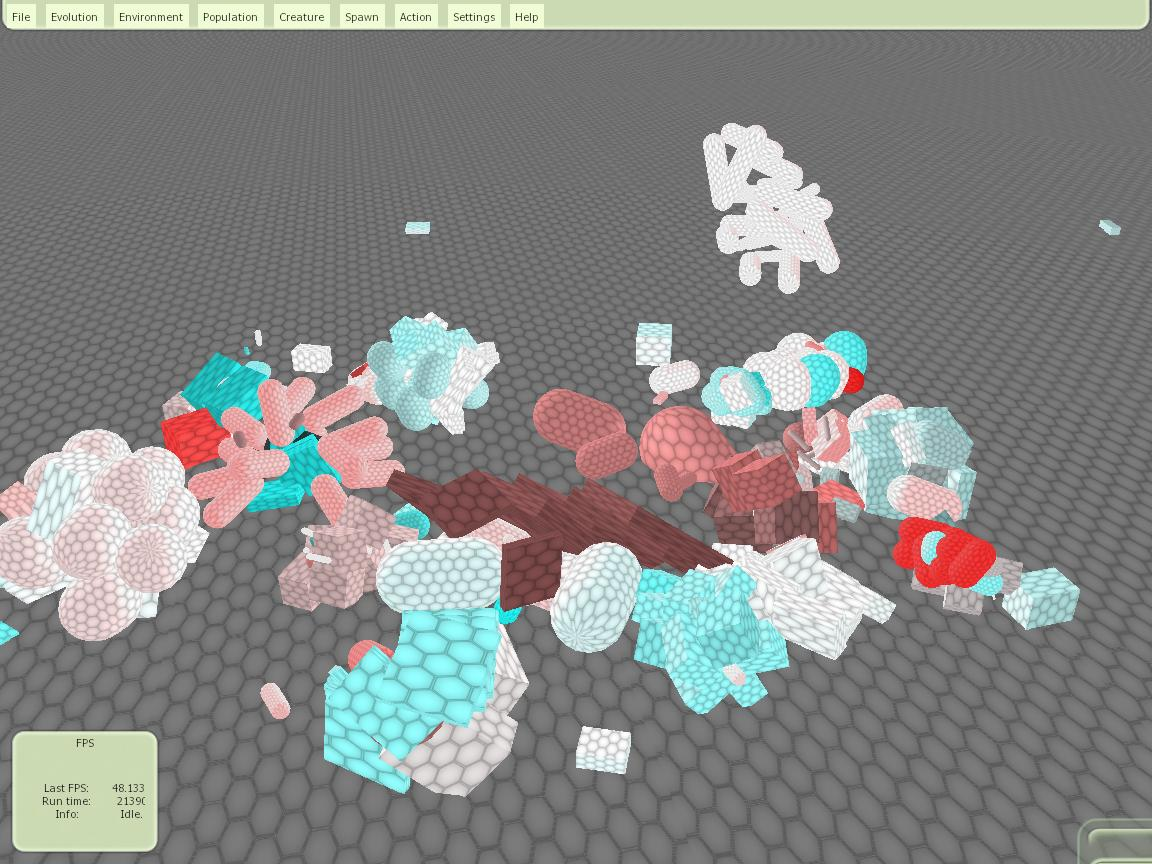
\includegraphics[width=3in, clip] {figs/creatures/Minemonics-05112015_190947481.jpg}
\end{figure}
  }
\note{}

\frame{

  \frametitle{Creatures}
  \begin{figure}[tp]
    \centering
    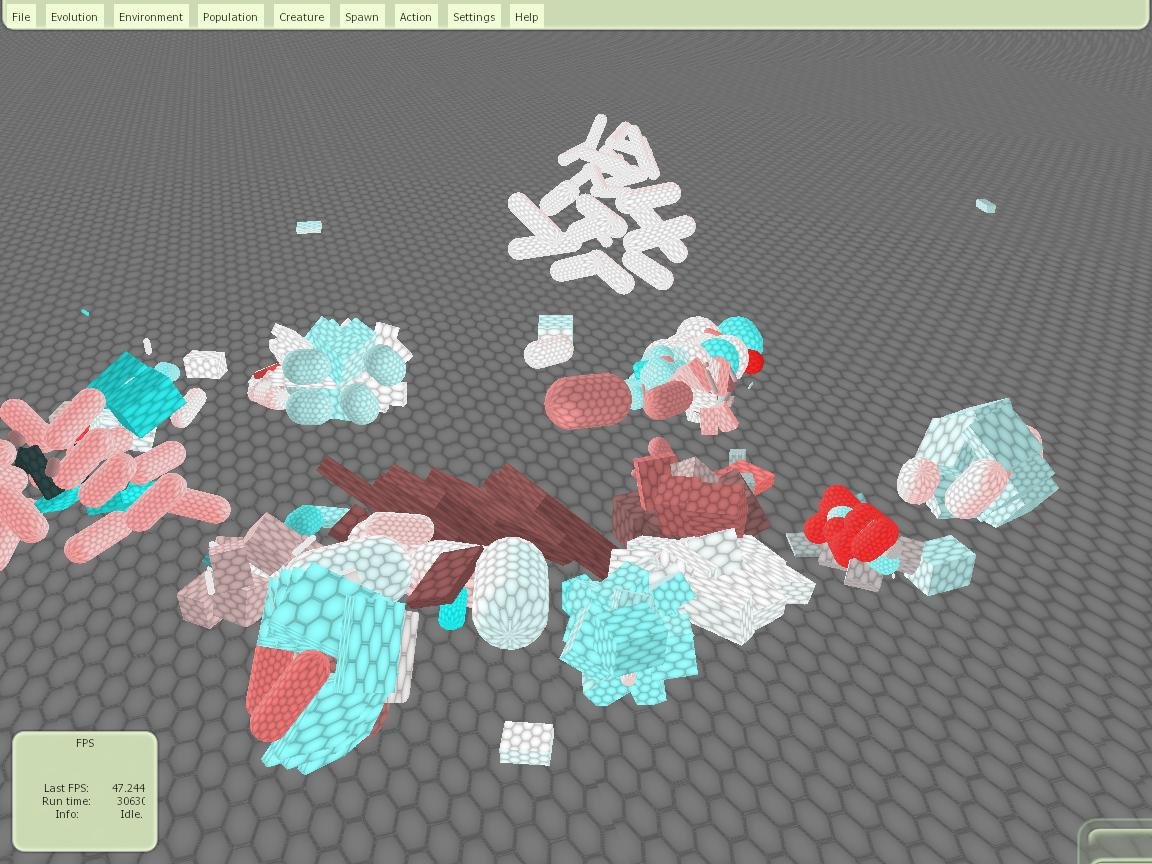
\includegraphics[width=3in, clip] {figs/creatures/Minemonics-05112015_190956720.jpg}
\end{figure}
  }
\note{}

\frame{

  \frametitle{Creatures}
  \begin{figure}[tp]
    \centering
    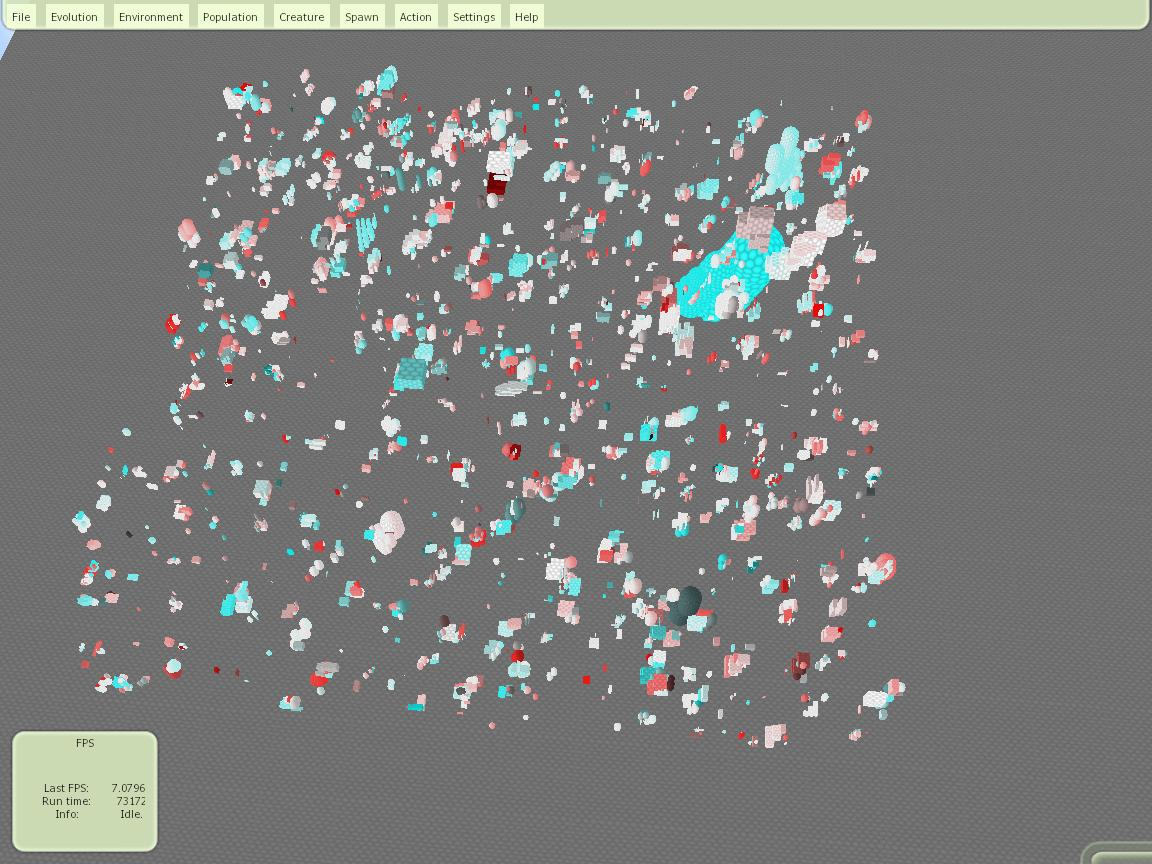
\includegraphics[width=3in, clip] {figs/creatures/Minemonics-05112015_191706383.jpg}
\end{figure}
  }
\note{}

\section{Outlook}

\frame{

  \frametitle{Contents}
    \tableofcontents[currentsection]
}
\note{}

\subsection{Optimization \& Extension}
\frame{

  \frametitle{Optimization \& Extension}
  
  \begin{itemize}
  \item The framework was written in a quick \& dirty manner
  \item Several components need to be reimplemented properly to provide a more scalable environment
  \item The system does not use any parallelization
  \item The phenotype could be more natural
  \item The genotype to phenotype transcription does not include any additional developmental parts (no embryogenesis)
  \item More sensor types
  \item More logging for data analysis
  \end{itemize}
}
\note{}
\subsection{Other settings \& fitness functions}
\frame{

  \frametitle{Other settings \& fitness functions}
  \begin{itemize}
  \item Island genetic algorithm
  \item Competitions of individuals
  \item Implicit fitness functions (survival of the fittest in a virtual world)
  \item Information theoretic measures such as the transfer entropy
  \end{itemize}
  
  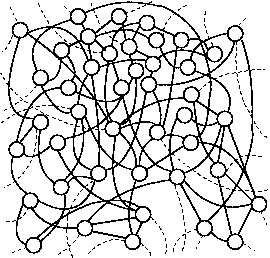
\includegraphics[width=1.5in, clip] {figs/NN.png} 
}
\note{}


\frame{

  \frametitle{References}
  \begin{itemize}
  \item Sims K. - Evolving Virtual Creatures (1994)
  \item Sims K. - Evolving 3D Morphology and Behavior by Competition (1994)
  \item Krcah P. - Evolving Virtual Creatures Revisited (2007)
  \item Schmidt N. - Bootstrapping perception using information theory: case studies in a quadruped running robot running on different grounds (2013)
  \item Hill, A.V. The heat of shortening and dynamics constants of muscles  (1938)
  \item Stoop R. - Theory and Simulation of Neural Networks (2014)
  \end{itemize}
}
\note{}



% Example slides
\begin{frame}
\textbf{Some mathematical specialities}

\ETHbox{0.8\textwidth}{% define the ETHbox
  \begin{theorem}[Murphy (1949)]\label{murphy}
    Anything that can go wrong, will go wrong.
  \end{theorem}
}

\begin{proof}
  A special case of Theorem \ref{murphy} is proven in %\citet{matthews1995}.
\end{proof}
\end{frame}

\begin{titlestyleframe}
\frametitle{Title Page}

\color{white} The title page is created using the \texttt{\textbackslash titleframe} command.

The title page background can also be used on other frames (or for a customised title frame) using the \texttt{titlestyleframe} environment.
\end{titlestyleframe}

\begin{frame}
\frametitle{Normal Frame}
The normal frame looks like this. It is created using the \texttt{frame} environment.
\end{frame}
\begin{inverseframe}
  \frametitle{Inverse Slides}
  %\color{white}
The inverted frame looks like this. It is created using the \texttt{inverseframe} environment.

 
\end{inverseframe}

\begin{minimalframe}
  \frametitle{Minimal Frame}
The minimal frame looks like this. It is created using the \texttt{minimalframe} environment.
  
\end{minimalframe}

\begin{frame}

\newcommand{\quadrat}{(0,0mm)--(0mm,5mm)--(5mm,5mm)--(5mm,0mm)--(0mm,0mm);}
\begin{center}
	\hspace{-8mm}
	\begin{tikzpicture}[overlay]
		{\draw[ETHa,fill=ETHa] \quadrat}\label{ETH1}
	\end{tikzpicture}
	\hspace{10mm}
	\begin{tikzpicture}[overlay]
		{\draw[ETHb,fill=ETHb]\quadrat}\label{ETH2}
	\end{tikzpicture}
	\hspace{10mm}
	\begin{tikzpicture}[overlay]
		{\draw[ETHc,fill=ETHc]\quadrat}\label{ETH3}
	\end{tikzpicture}
	\hspace{10mm}
	\begin{tikzpicture}[overlay]
		{\draw[ETHd,fill=ETHd] \quadrat}\label{ETH4}
	\end{tikzpicture}
	\hspace{10mm}
	\begin{tikzpicture}[overlay]
		{\draw[ETHe,fill=ETHe] \quadrat}\label{ETH5}
	\end{tikzpicture}
	\hspace{10mm}
	\begin{tikzpicture}[overlay]
		{\draw[ETHf,fill=ETHf] \quadrat}\label{ETH6}
	\end{tikzpicture}
	\hspace{10mm}
	\begin{tikzpicture}[overlay]
		{\draw[ETHg,fill=ETHg] \quadrat}\label{ETH7}
	\end{tikzpicture}
	\hspace{10mm}
	\begin{tikzpicture}[overlay]
		{\draw[ETHh,fill=ETHh] \quadrat}\label{ETH8}
	\end{tikzpicture}
	\hspace{10mm}
	\begin{tikzpicture}[overlay]
		{\draw[ETHi,fill=ETHi] \quadrat}\label{ETH9}
	\end{tikzpicture}
\end{center}

\end{frame}

\end{document}
